\documentclass[10pt]{scrartcl}

\usepackage{graphicx}
\usepackage{subcaption} 

\title{Scientific Experimentation and Evaluation\\
	   \small{Assignment: 1}}
\author{Chaitanya Hebbal\\
		Jos\'e Carlos Mayoral Ba\~nos}

\begin{document}
	\maketitle
\section*{Task Description}

Our \textbf{task} is defined as: \textit{Constructing a LEGO NxT differential drive robot and manually measure the observable pose variation for three different velocity motions}. The goal of this experiment is to observe the variation on the manual measured poses and look at the error distributions.

%In order to achieved the goal, there are some constraints that must be taken into account:

%\begin{itemize}
%	\item The Device Under Test is a LEGO NxT robot.
%	\item DifferentialPilot library for motion behaviour.
%	\item Manual measurement comes out with additional error provided by the person who makes them.
%	\item The time of every movement must be constant.
%	\item There is not a true value to compare with, this must be obtained from the repetitions of the experiment.
%\end{itemize}

The layout of this experiment consists on:
\begin{enumerate}
%	\item DifferentialPilot library for motion behaviour.
%	\item Manual measurement comes out with additional error provided by the person who makes them.
%	\item The time of every movement must be constant.
%	\item There is not a true value to compare with, this must be obtained from the repetitions of the experiment.
	\item Five different curves movements are going to be measured: Straight line and 4 arcs (2 left and 2 right).
	\item The Device Under Test is a LEGO NxT robot.
	\item A third-part library for the software is previously defined.
\end{enumerate}

Plan for the experiment is given below:

\begin{enumerate}
	\item Define the measurement method (see below).
	\item Code a good program which takes into consideration the provided restrictions.
	\item Define the curves that must be done according to pre-defined library.
	\item Store the information of the final poses.
	\item Repeat twenty times every curve measurement.
	\item Compute the information to get the error gaussian distribution.
\end{enumerate}
\section*{Experiment setup}

\subsection*{Device Under Test}

The Device Under Test is a LEGO NxT robot, shown at figure \ref{fig:1}.

\begin{figure}[h!]
\centering
\caption{LEGO Nxt Robot}
\label{fig:1}
  \begin{subfigure}[b]{0.4\textwidth}
    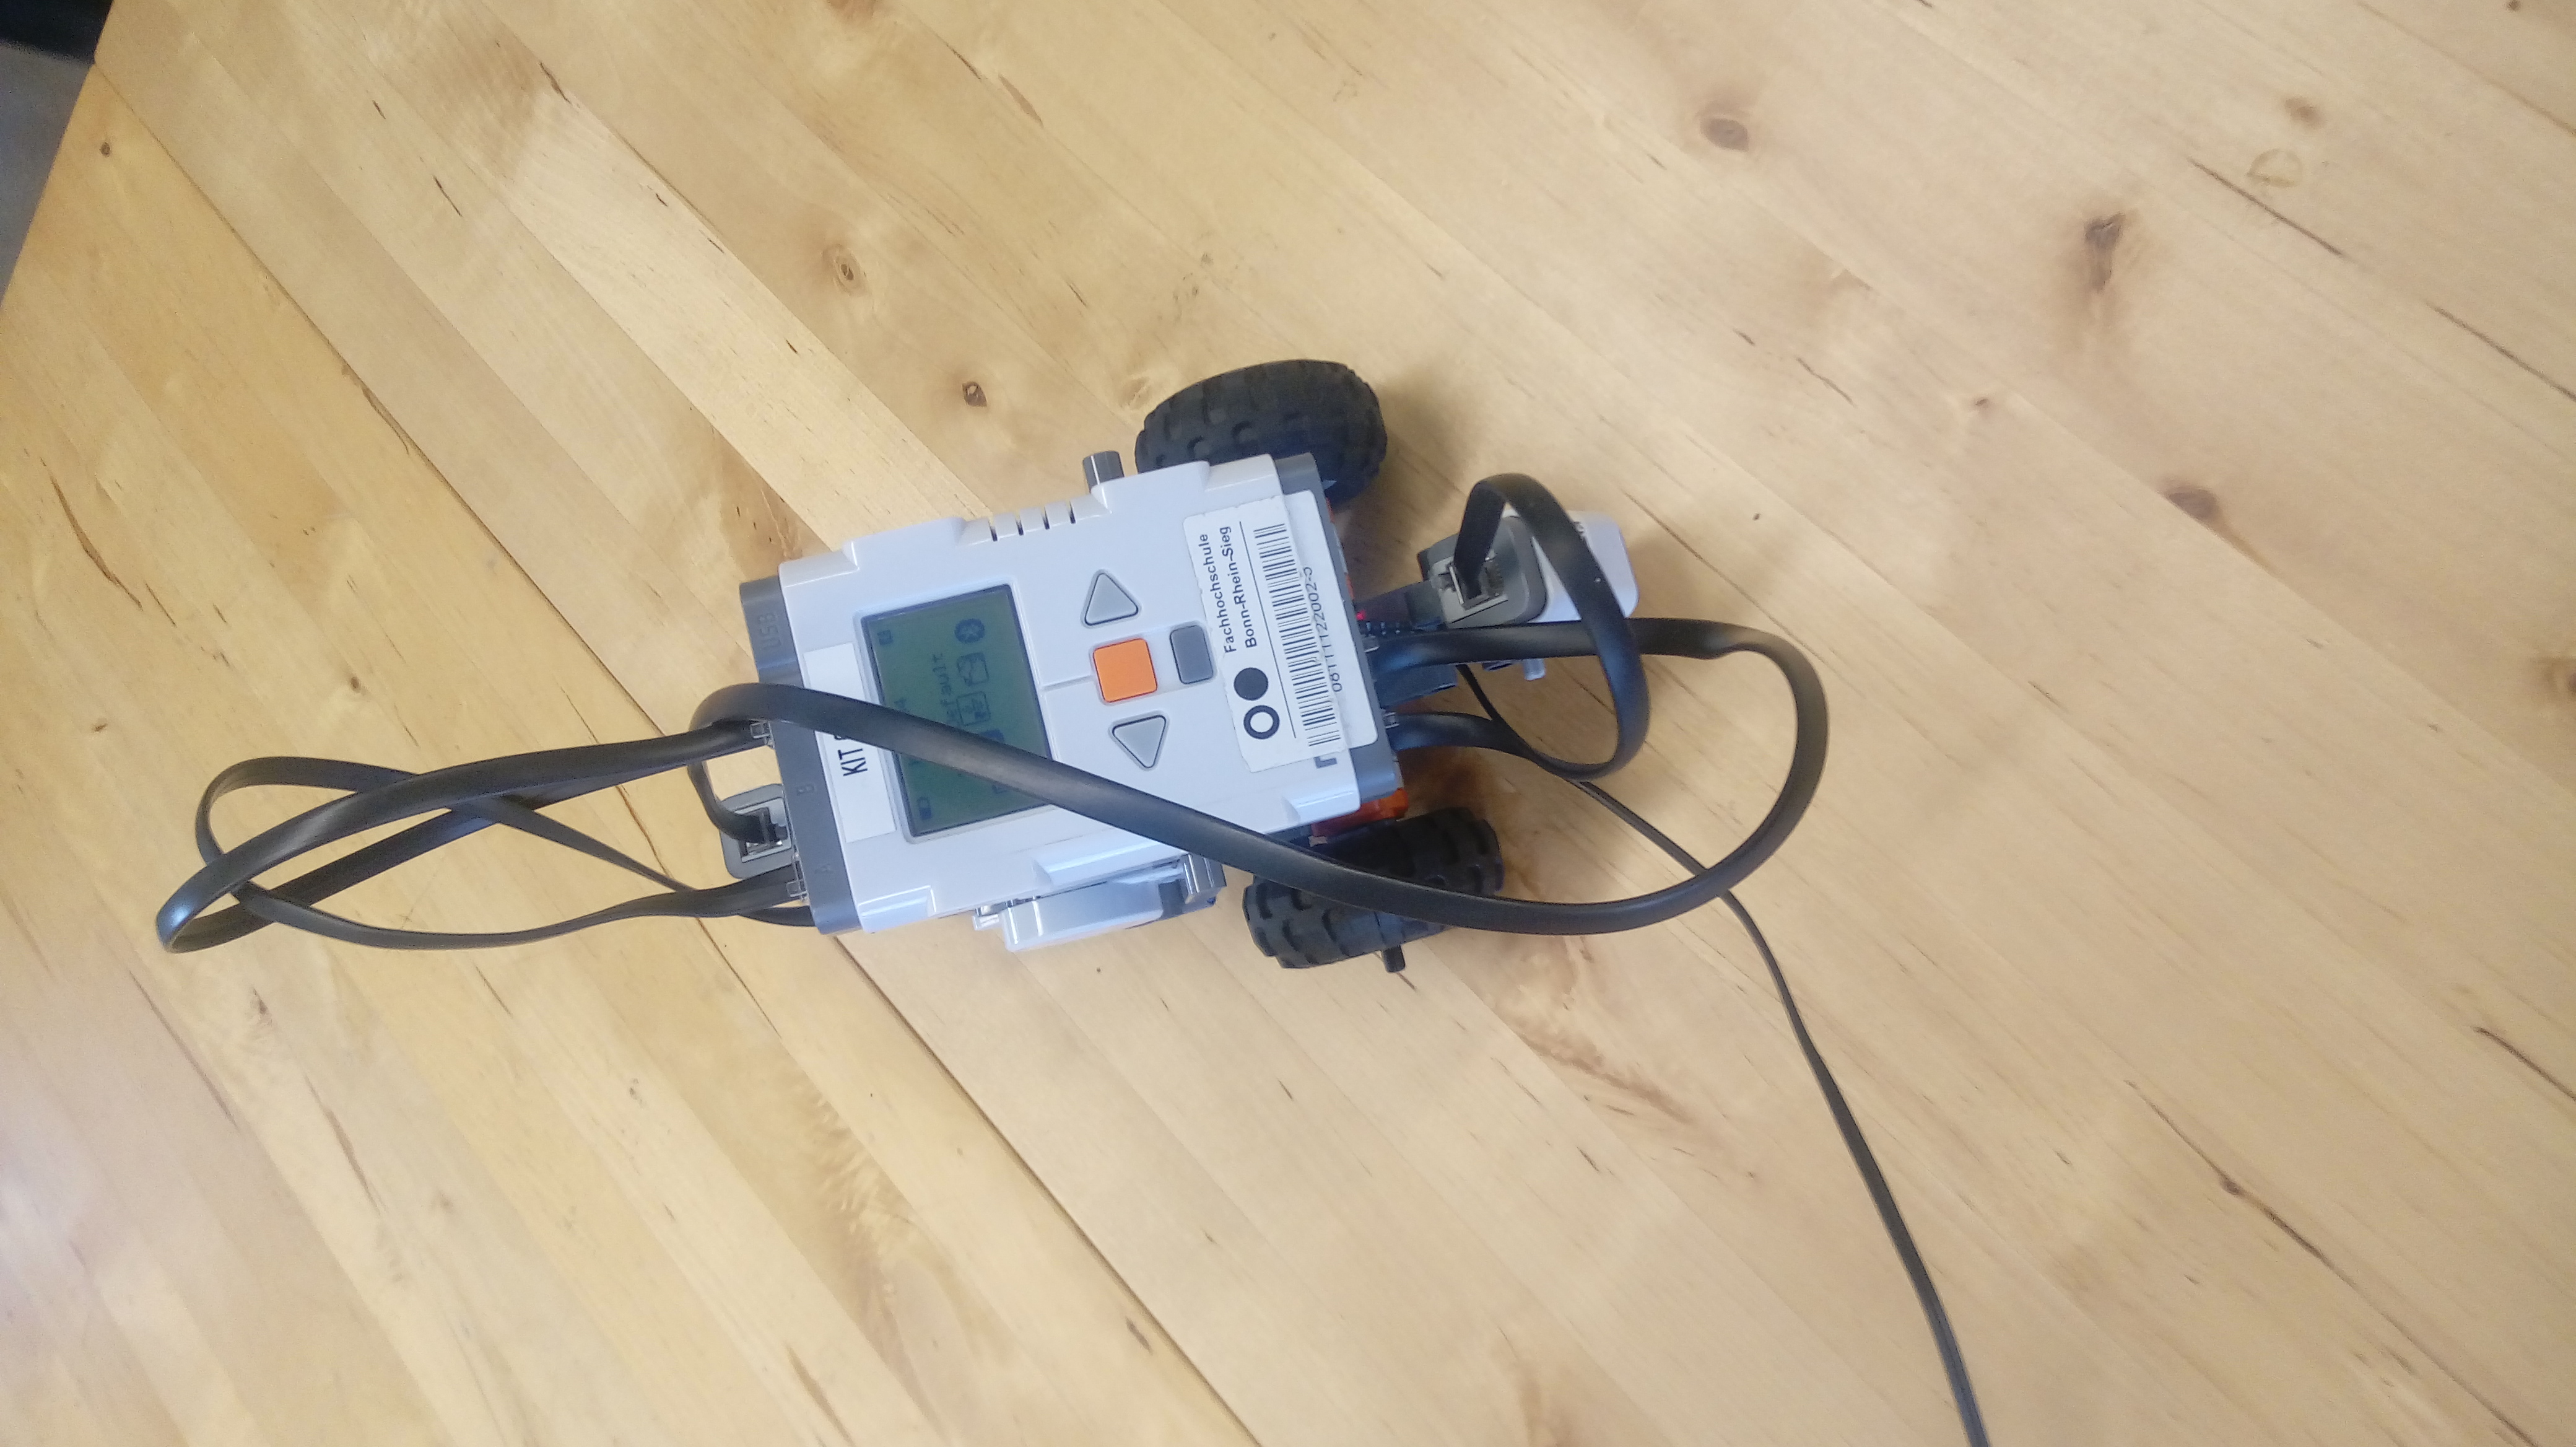
\includegraphics[width=\textwidth]{images/robot_1}
    %\caption{Picture 1}
    %\label{fig:1}
  \end{subfigure}
  %
  \begin{subfigure}[b]{0.4\textwidth}
    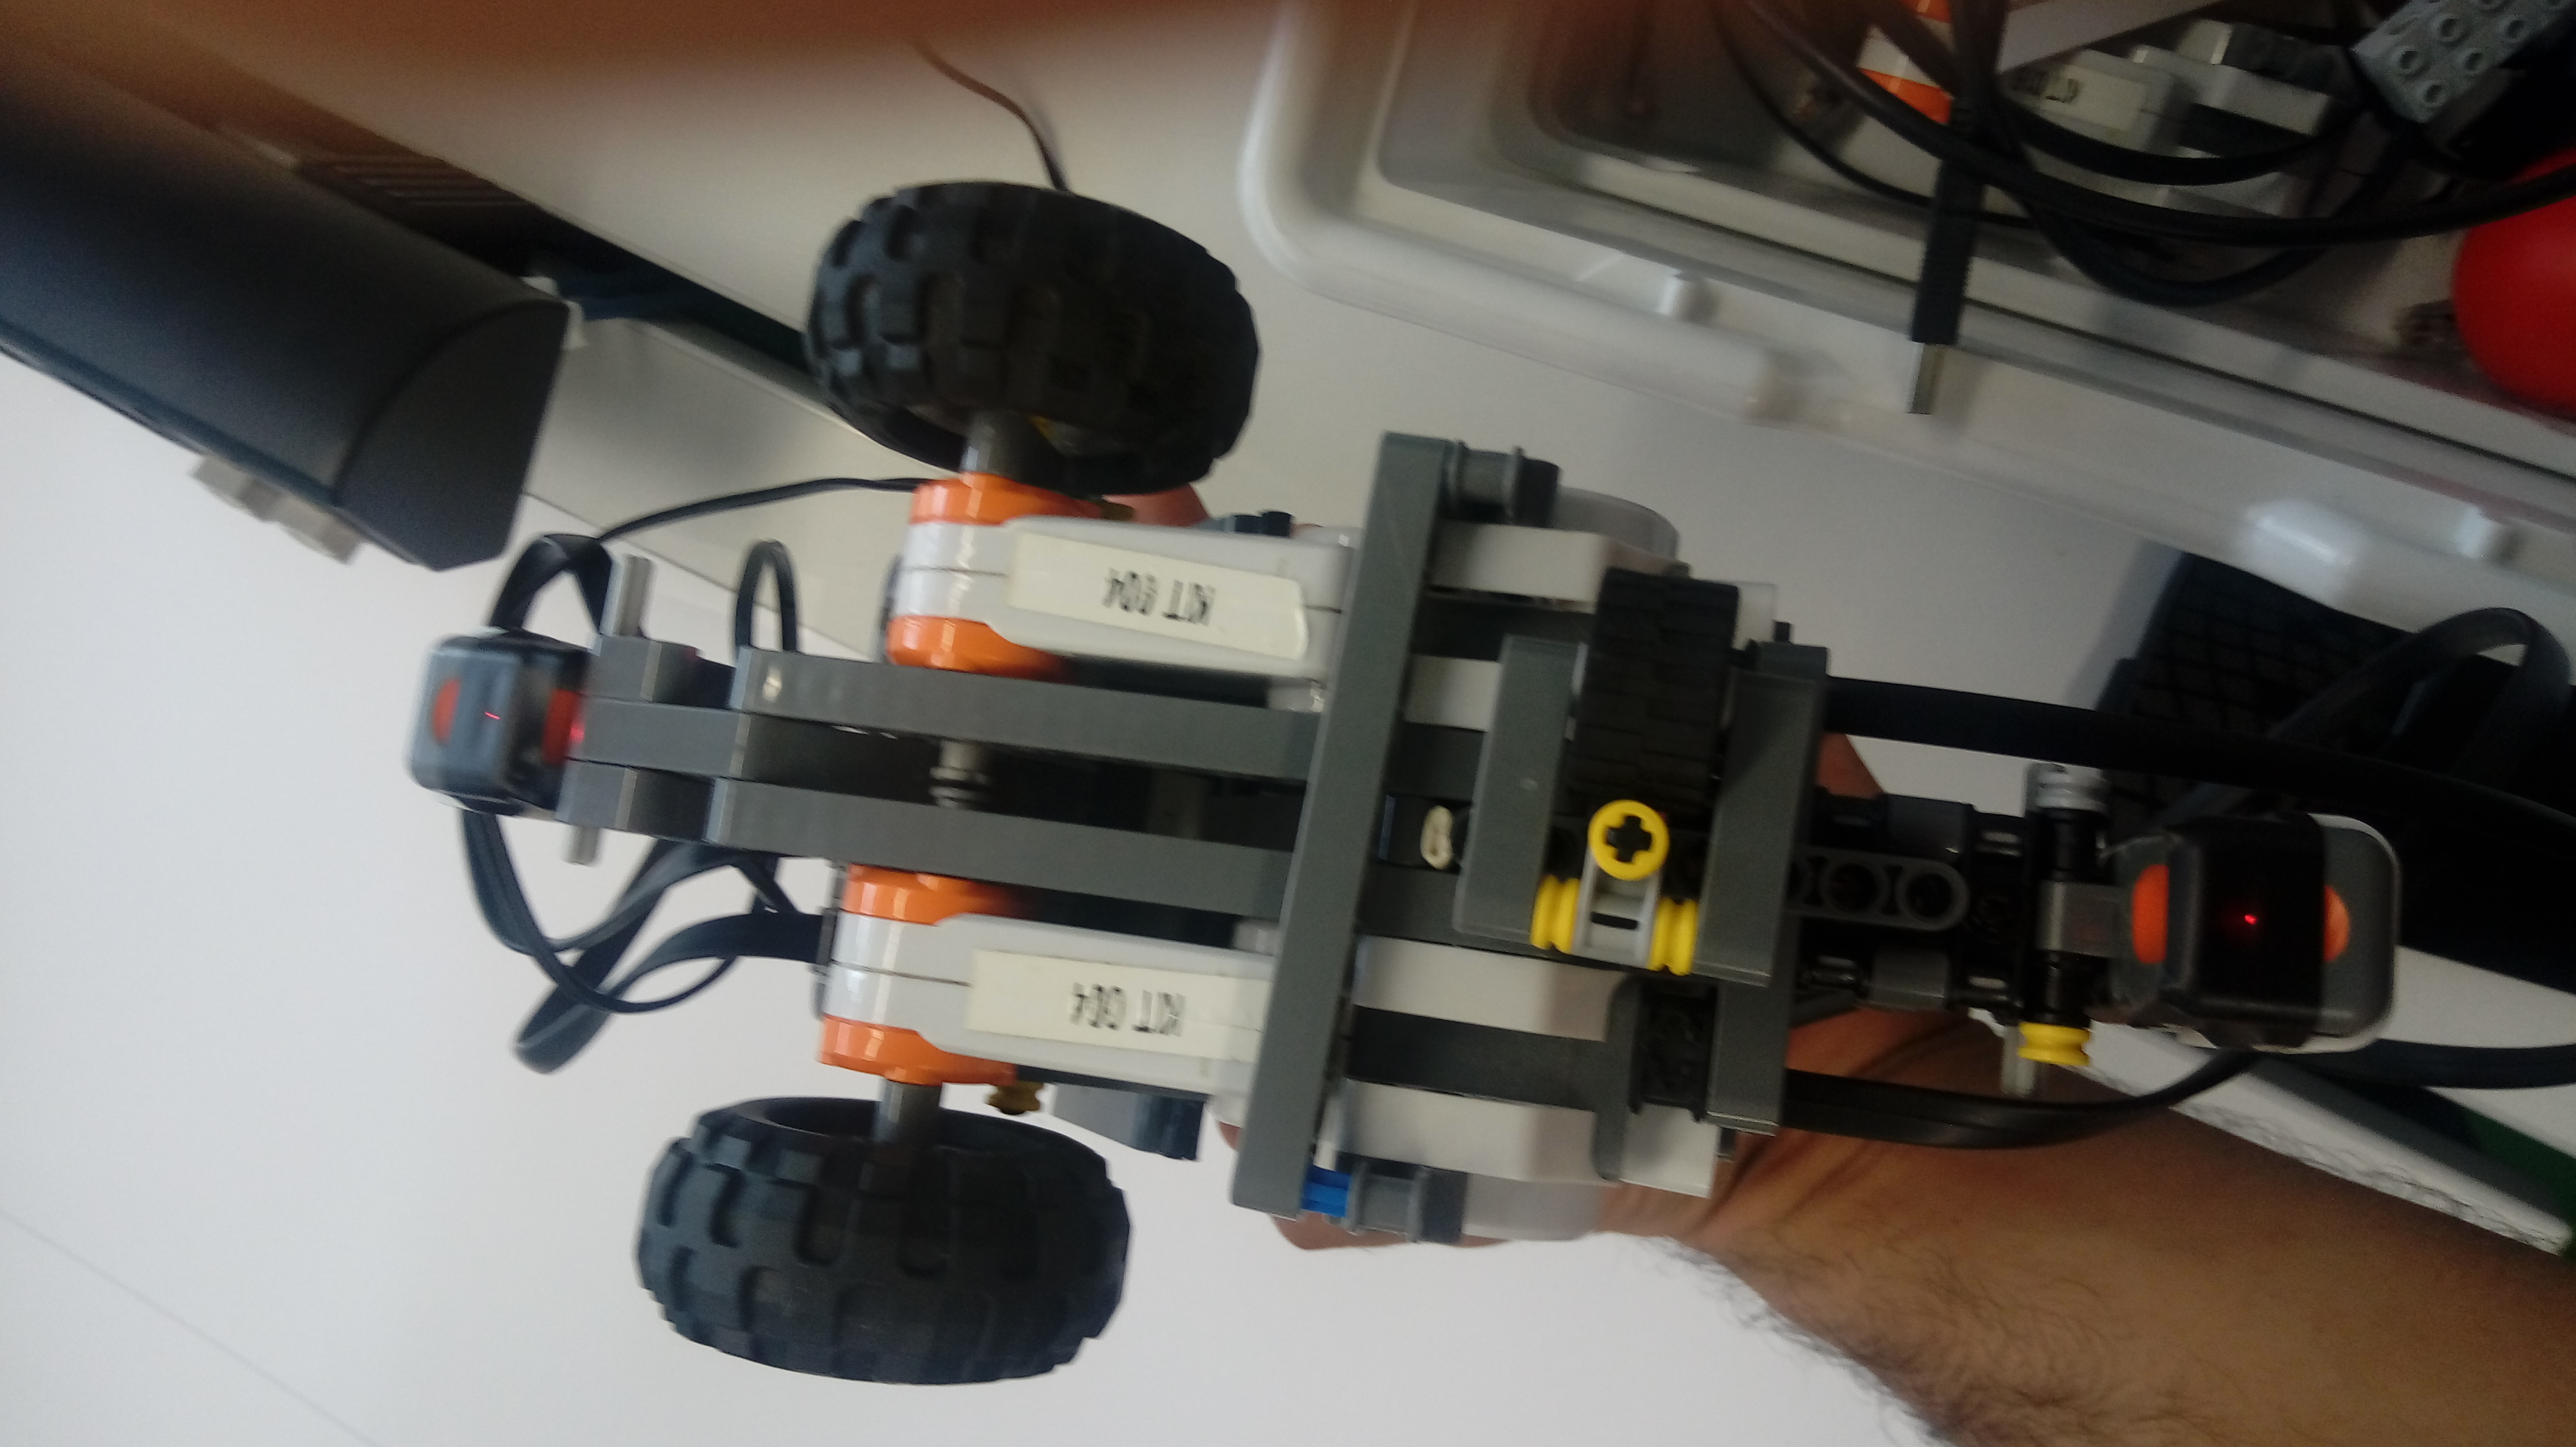
\includegraphics[width=\textwidth]{images/robot_2}
	%\caption{Picture 2}
    %\label{fig:2}
  \end{subfigure}
\end{figure}

\subsection*{Measured Value}
The polar coordinate of the robot (distance to origin, and angle $ \theta $).

\subsection*{Measurement System}

The measurement value (final pose) is acquired by a LEGO NxT robot which uses the libraries provided by leJOS framework for motion and a large cardboard sheet, light sensor and geometric representation to acquire data. 

\subsection*{Measuring Method}

To accomplish the task we have defined the experiment as explained in the picture.\\

\begin{figure}[h!]
\centering
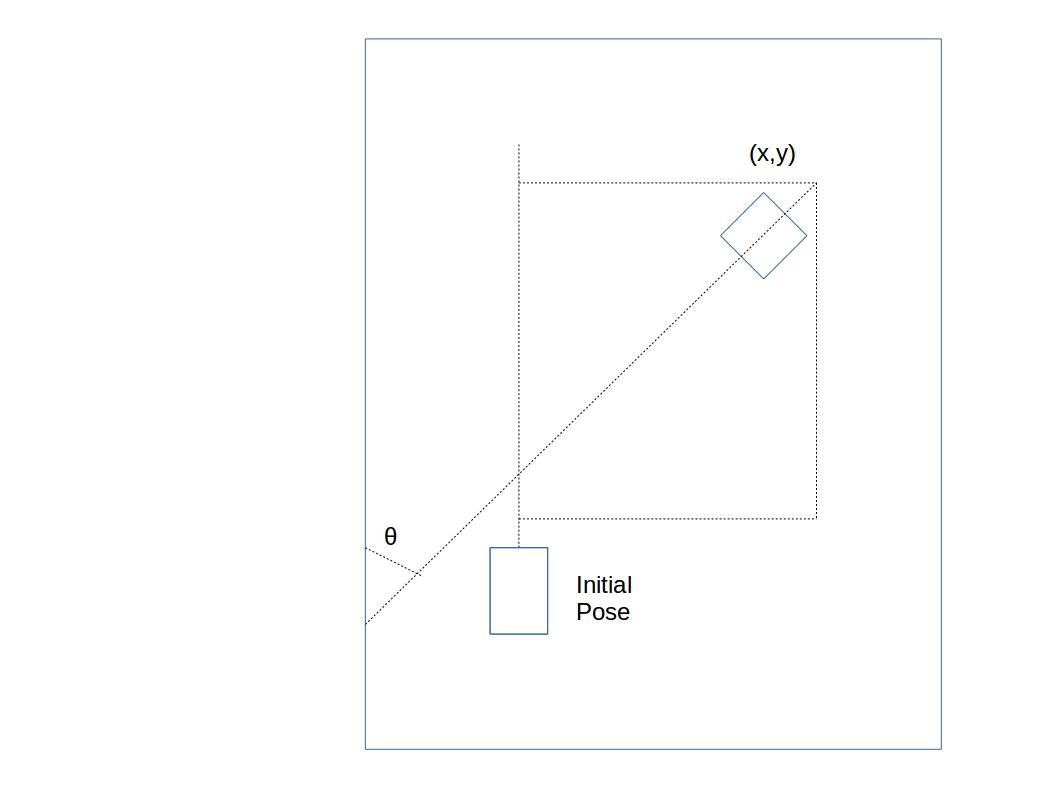
\includegraphics[trim=200 0 0 0, scale=0.35]{images/image}
\caption{Experiment Description}
\label{fig:3}
\end{figure}

The method description of image \ref{fig:3} is:
\begin{itemize}
	%\item One LEGO structure will set the robot at initial position so the initial position will be constant.
	\item A cardboard is used to mark the points of all the experiment.
	\item Two light sensors are used to mark the points in order to get the pose of the robot.
	\item Using LEGO light sensors initial pose is marked on the cardboard.
	\item A perpendicular axis which connects two original points is drawn as a reference.
	\item The origin is located between wheels so there distance from a sensor to the center must be measured. 
	\item After the robot stops, a projection of the line is drawn between the two measured points pointed by the sensors.
	\item The angle will be measured between the reference axis and the projected line.
	\item From the final marks, the new center is calculating extracting distance from initial marker to center along the projected line.
	\item Linear distance comes from the distance between measured center the and origin.
	\item For every repetition the initial pose must fit the original pose markers.	
	\item After 5 repetitions, erase marks in order to get better measurements.
\end{itemize}

The Measurement facilities include:

\begin{itemize}
	\item One cardboard.
	\item Two light sensors.
	\item A pen.
	\item A protractor.
	\item A rule.
\end{itemize}

The used light markers use is shown at image \ref{fig:4}.
\begin{figure}[h!]
\centering
\caption{LEGO Nxt Robot Light Markers}
\label{fig:4}
  \begin{subfigure}[b]{0.4\textwidth}
    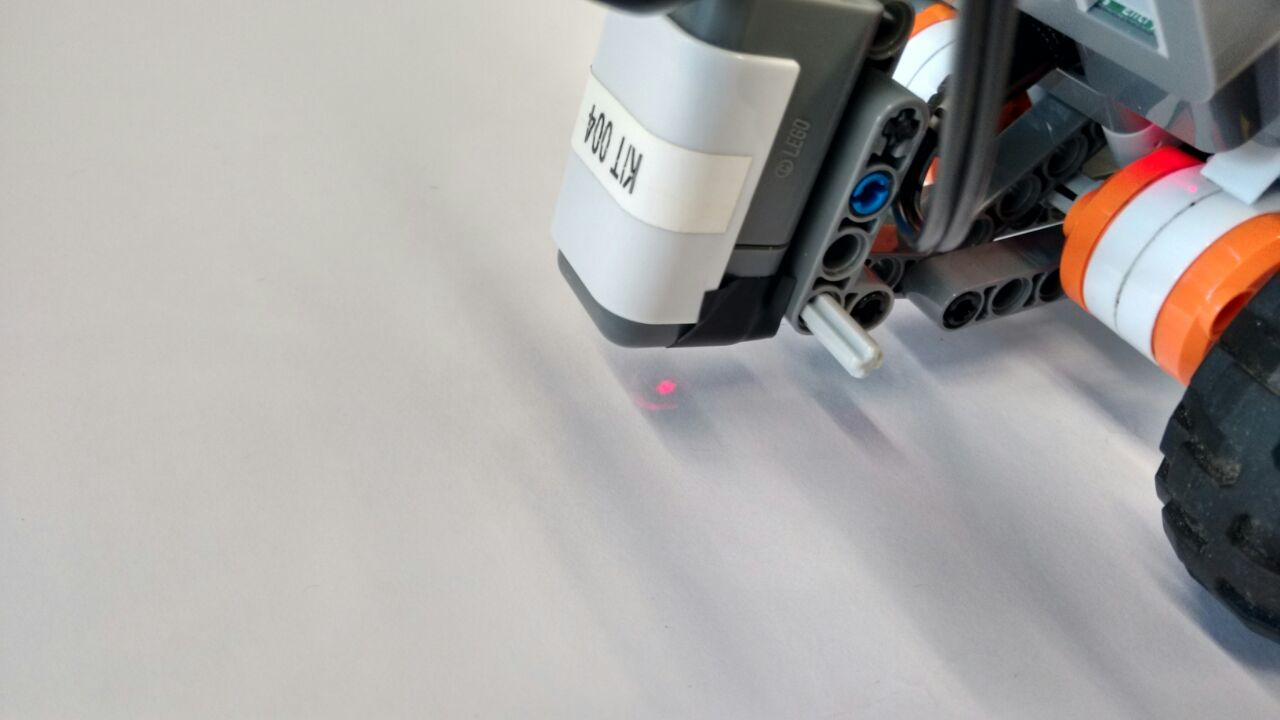
\includegraphics[width=\textwidth]{images/marker_1}
	\caption{Forward Marker}
	
  \end{subfigure}
  %
  \begin{subfigure}[b]{0.4\textwidth}
    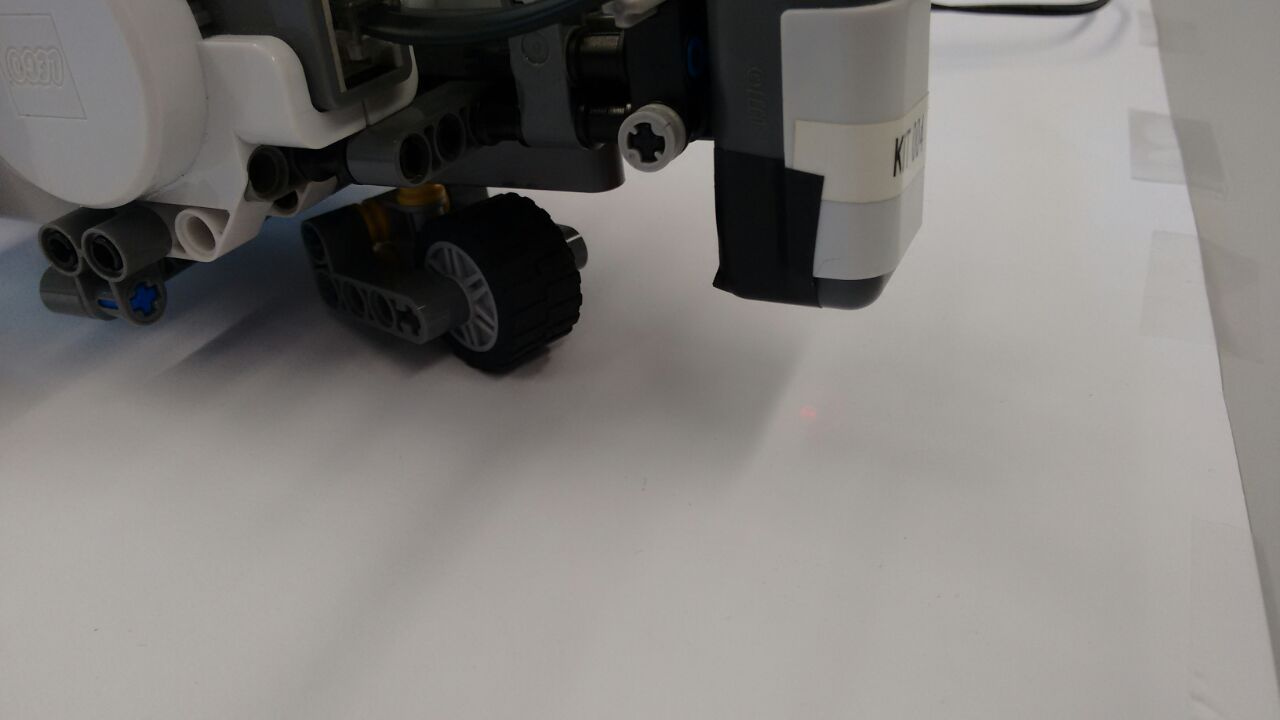
\includegraphics[width=\textwidth]{images/marker_2}
	\caption{Backward Marker}
  \end{subfigure}
\end{figure}


\subsection*{What difficulties are expected?}

In order to accomplish the current task, we found the following constraints:

\begin{itemize}
	\item The manual measurement will add errors to the measurement result.
	\item The precision of the instruments will affect the gaussian distribution.
\end{itemize}

\section*{Experimental Observations}

An example of the measurement process can be seen at figure \ref{fig:6}. 

\begin{figure}[h!]
\centering
\caption{Measurement Process}
\label{fig:6}
  \begin{subfigure}[b]{0.4\textwidth}
    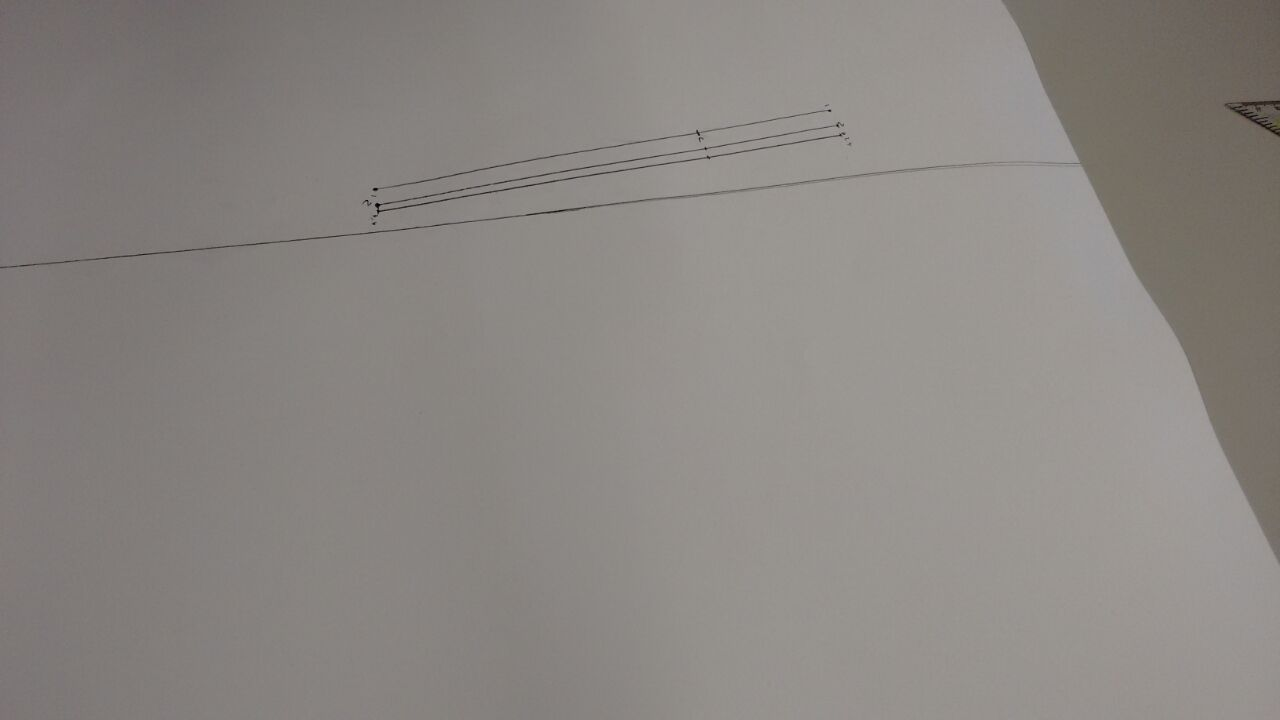
\includegraphics[width=\textwidth]{images/measurements}
    %\caption{Picture 1}
  \end{subfigure}
\end{figure}

The right motor seems to be steeper as the left one, i.e. the straight line deviates to left (image \ref{fig:7}).

\begin{figure}[h!]
\centering
\caption{Experiments print}
\label{fig:7}
  \begin{subfigure}[b]{0.8\textwidth}
    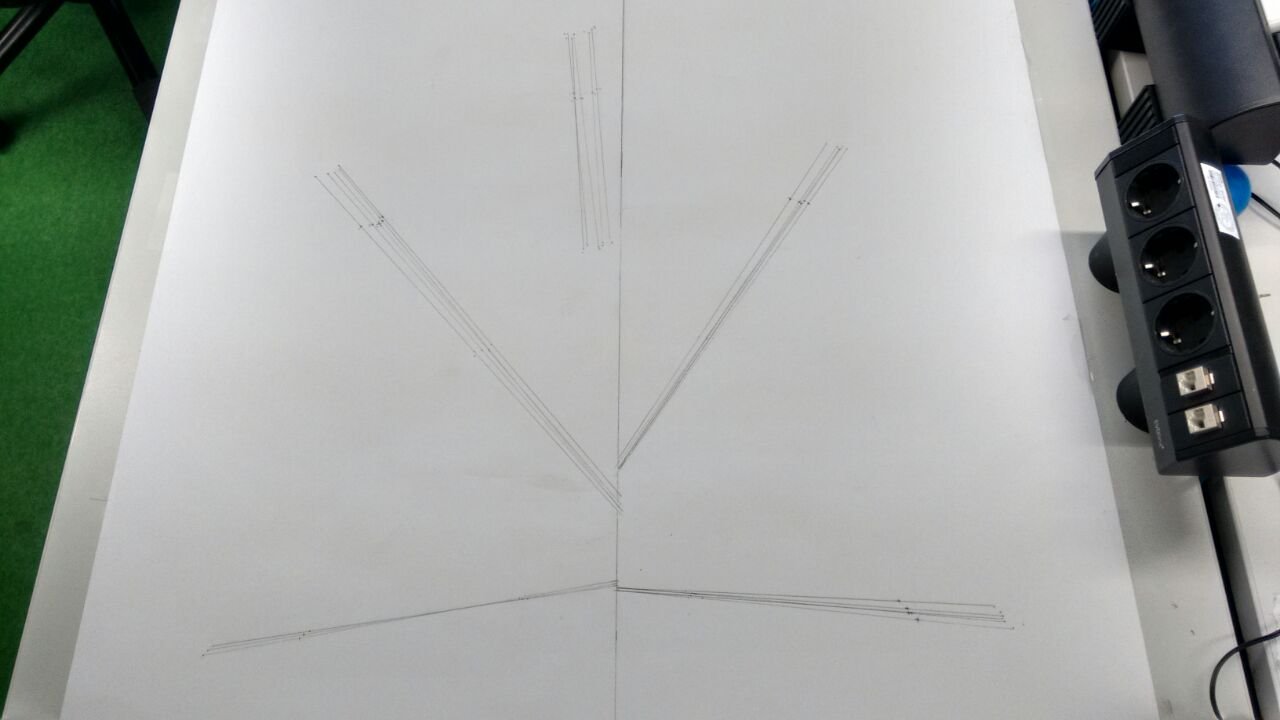
\includegraphics[width=\textwidth]{images/print}
    %\caption{Picture 1}
  \end{subfigure}
\end{figure}

The experiments results are provided in the attached file: $"see\_data\_.ods"$.

\subsection*{Precision and Accuracy}

The precision of the experiment relies on the precision of the measurement facilities:
\begin{itemize}
	\item For Distance Measurement: the rule was used which precision is 1 mm.
	\item For Angle Measurement: the protractor was used which precision is 1$^{\circ}$.
\end{itemize}

\newpage
\subsection*{Parameters used to drive the robot}

\begin{table}[ht!]
\centering
\caption{Parameters Used}
\label{params}
\begin{tabular}{|c|c|c|c|c|} \hline
 				& Arc radius& Angle & Distance & Track Width \\ \hline
Steep left arc  & 20        & 90    &          & 12 \\ \hline
Steep right arc & 20        & 90    &          & 12 \\ \hline
Soft left arc   &           & 40    & 55       & 12 \\ \hline
Soft right arc  &           & 40    & 55       & 12 \\ \hline
Straight        & 40        & 90    &          & 12 \\ \hline
 
\end{tabular}
\end{table}

	
\end{document}